
% This overabundance of ribosomes
% provides different challenges on the ability of the cell to maintain steady-state
% growth under limiting nutrient conditions, and in Supplemental
% Section XX we consider this slow growth regime further.

% While this dependence between cell size and ribosomal abundance is apparent
% across moderate to fast growth rates, it is worth noting that

% This scaling behavior is likely to change at slow growth rates (below $\lambda
% \approx 0.5\,\text{hr}^{-1}$). Here, the number of ribosomes $R$ no longer
% reflects the cell's protein synthesis capacity, so far taken to be $r_t \ R$.
% Instead, cells reduce the number of actively translating ribosomes through the
% additional regulatory control of the small-molecule alarmone, guanosine
% pentaphosphate [(p)ppGpp] \citep{dai2016} [more citations].

% \subsection{Ribosomal Elongation Rate and Cellular Growth Rate are Linked by Amino Acid Scarcity}
\subsection{Alarmone-Mediated Regulation Controls the Rate of Protein Synthesis}

As we have seen, cell size, number of actively translating ribosomes, and
cellular growth rate are intimately connected. This provides a mechanistic
framework through which we can understand how cellular physiology is tuned to
match biosynthetic capacity to the nutrient conditions of the environment. Take,
for example, the recent experimental work by \cite{dai2016} which measured the
perturbation to these key cellular phenotypes resulting from deletion of the
primary glucose transport system in \textit{E. coli}. In this deletion
background, \textit{both} cellular growth rate \textit{and} the ribosome mass fraction of the
proteome decreased by a factor of two relative to a strain with wild-type levels
of the glucose transporters. This factor of two decrease in growth rate
is agreement with the intuition provided by \EQ{translation_limit_growth_rate}
for a ribosome mass fraction decrease of this magnitude. In the final section of
this work, we explore the interconnection between cell size, ribosome content,
and growth rate from a mathematical perspective, resulting in a minimal model
of growth rate regulation given the nutrient conditions of the growth medium.

% suggest that cell size and ribosome content is tuned as a means
% to match the biosynthetic capacity to the available nutrient conditions. An
% illustration of this principle can be seen in the recent work of
% \cite{dai2016} where disruption of the major glucose uptake system through
% the deletion of \textit{ptsG} limits carbon uptake and growth by a factor of
% two as well as reduces the ribosomal mass fraction by a factor of two. and
% growth, which is reduced about two-fold. This matches our intuition given a
% decrease in growth rate governed by \EQ{translation_limit_growth_rate} for a
% change in ribosomal fraction of this magnitude. In this final section, we
% formulate and explore a minimal model of growth rate control. We use it to
% quantitatively show how changes in ribosomal content and total proteomic mass
% will allow cells to maximize their growth rate according to the available
% nutrient conditions, which we generalize as a supply of amino acids.

To react to changes in nutrient conditions, bacteria rely on
the synthesis or degradation of secondary-messenger molecules termed alarmones
like guanosine pentaphosphate [(p)ppGpp], which result in changes to the global
transcriptional and translational activity. In \textit{E. coli}, amino acid
starvation causes the accumulation of de-acylated tRNAs at the ribosome's
A-site, leading to a strong increase in (p)ppGpp synthesis activity by the
enzyme RelA\citep{hauryliuk2015}. The accumulation of (p)ppGpp regulates the
fraction of the ribosome pool which is actively translating, $f_a$. The
concentration of (p)ppGpp increases as growth rate is slowed (with $f_a \approx
0.5$ at a growth rate of $\approx$ 0.3 hr$^{-1}$), indicating that regulation of
ribosome activity is linked to coordinating growth in poor nutrient conditions.

Furthermore, (p)ppGpp can inhibit the initiation of DNA
replication by mediating a change in transcriptional activity and the
supercoiling state of the origin of replication \citep{kraemer2019}. These
observations all raise the possibility that, via (p)ppGpp, cells mediate the
growth-rate dependent changes in $\langle$\# ori$\rangle$, cell size and
ribosomal abundance \citep{zhu2019, Buke2020}. Indeed, recent work in a
(p)ppGpp deficient strain of \textit{E. coli} found that cells exhibited a
high ratio of $\langle$\# ori$\rangle$ to $\langle$\# ter$\rangle$ and cell
size that was more consistent with a fast growth state where (p)ppGpp levels
are normally low \citep{fernandezcoll2020}.

\subsection{Ribosomal Elongation Rate and Cellular Growth Rate are Linked by Amino Acid Scarcity}
To better understand how cells are able to maximize their growth rate under
different degrees of nutrient limitation, we consider a mode of regulation in
which the rate of peptide elongation $r_t$ depends only on the availability
of amino acids (and, therefore, also amino-acyl tRNAs). As the rate of amino
acid supply $r_{AA}$ decreases, slowing the rate of elongation provides a
means by which the cell can tune the rate of amino acid consumption
(mathematized as $r_t \times R \times f_a$) to remain in steady-state growth,
shown schematically in \FIG{elongation_rate_model}(A). Under this simplistic
model, other molecular players required for translation like elongation
factors and GTP are considered in sufficient abundance, which appear to be
valid assumptions given our analysis of the proteomic data and energy
production thus far.

For simplicity, we consider all amino acids as a single
species with an effective cellular concentration $[AA]_\text{eff}$. The
rate of elongation $r_t$ will depend on how quickly the ribosomes can match
codons with their correct amino-acyl tRNA, along with the subsequent steps of
peptide bond formation and translocation. We therefore coarse-grain the steps of
elongation to two time-scales,  1) the time required
to find and bind each correct amino-acyl tRNA, and 2) the remaining steps in
peptide elongation that will not depend on the amino acid availability. The
time to translate each codon is given by the inverse of the elongation rate
$r_t$, which can be written as,

\begin{equation}
\frac{1}{r_t} = \frac{1}{k_{on} \alpha [AA]_{\text{eff}}} + \frac{1}{r_{t}^{\text{max}}}.
\end{equation}
where we have assumed that the rate of binding by amino-acyl tRNA $k_{on}$ is
proportional to $[AA]_{\text{eff}}$ by a constant $\alpha$. The second term on the
right-hand side reflects our assumption that other steps in peptide elongation
are not rate-limiting, with a maximum elongation rate $r_{t}^{\text{max}}$ of
about 17 amino acids per second \cite{dai2016}. This can be stated more succinctly in
terms of an effective dissociation constant,

\begin{equation}
    K_D = \frac{r_{t}^{\text{max}}}{\alpha k_\text{on}},
\end{equation}
where the elongation rate $r_t$ is now given by

\begin{equation}
r_t = \frac{r_{t}^{\text{max}}}{1 + K_D/[AA]_{\text{eff}}}.
\label{eq:rt_kd_simple}
\end{equation}

Under steady-state growth, the amino acid concentration is constant
($\frac{d[AA]_\text{eff}}{dt}=0$), meaning that synthesis and consumption are matched.
The effective amino acid concentration $[AA]_{\text{eff}}$ will relate to the rate of
amino acid synthesis (or import, for rich media) and/or tRNA charging, 
as $r_{AA}$,  and the rate of consumption,
$r_t\times R \times f_a$ by,

\begin{equation}
\int_{0}^{t} \frac{d[AA]_{\text{eff}}}{dt} dt =  \int_{0}^{t}([r_{AA}] - [r_t\times R \times f_a]) dt,
\label{eq:aaeff_int}
\end{equation}
where the time from 0 to $t$ is an arbitrary length of time, and the square
brackets indicate concentrations per unit time. 
Integrating \EQ{aaeff_int} yields.
\begin{equation}
[AA]_{\text{eff}} =  t([r_{AA}] - [r_t \times R \times f_a]).
\label{eq:aaeff_concs}
\end{equation}

Alternatively, we can state this in terms of absolute ribosome copy number $R$
by considering a unit volume $V$,
\begin{equation}
   [AA]_\text{eff} = \frac{t(r_{AA} - r_t \times R \times f_a)}{V},
   \label{eq:aa_final}
\end{equation} 
where $r_{AA}$ is in units of AA per unit time and $r_t$ is in units of AA per
unit time per ribosome. With an expression for $[AA]_\text{eff}$ in hand, we can now solve
\EQ{rt_kd_simple} for $r_t$ which is a quadratic function with a
physically-meaningful positive root of
\begin{equation}
r_t = \frac{-t(r_{AA} + r_t^\text{(max)}Rf_a) - K_D V \pm \sqrt{(r_{AA}t + r_t^\text{(max)}Rf_at + K_D V)^2 - 4(Rf_at)(r_t^\text{(max)}r_{AA} t)}}{-2Rf_at}.
\label{eq:rt_root}
\end{equation}

In \FIG{elongation_rate_model}(B), we illustrate how the elongation rate depends
on the ribosomal copy number. Here, we have considered a unit volume $V =
1$\textmu m$^3$, a unit time $t = 1$ s, a $K_D = 5$ mM (inferred from
\cite{bennett2009}), $f_a = 1$, and an arbitrarily chosen $r_{AA} = 5\times 10^6$ AA
$\cdot$ s$^{-1} \cdot$ \textmu m$^{-3}$. At low ribosome copy numbers, the
observed elongation rate is dependent primarily on the ratio of $K_D / Vr_{AA}$
[as $r_t^{\text{max}} \times R \times f_a << r_{AA}$, point (1) in
\FIG{elongation_rate_model}(B)]. As the ribosome copy number is increased such
that the amino acid supply rate and  consumption rate are nearly equal [point
(2) in \FIG{elongation_rate_model}(B)], the observed elongation rate begins to
decrease sharply. When the ribosome copy number is increased even further,
consumption at the maximum elongation rate exceeds the supply rate, yielding  a
significantly reduced elongation rate [point (3) in
\FIG{elongation_rate_model}{B)]. While the elongation rate will always be
dominated by the amino acid supply rate at sufficiently low ribosome copy
numbers, the elongation rate at larger ribosome abundances can be increased by
tuning $f_a$ such that not all ribosomes are elongating, reducing the total
consumption rate.  

It is important to note that thus far, this model quantifies only the
relationship between amino acid supply and consumption as a function of the
ribosome copy number and states nothing about the cellular growth rate, 
illustrating the separation of time scales in this minimal model. With a sense of
how elongation rate is tied to amino acid abundance, we now turn to how this
relates to the principal cellular phenotype of this work, the cellular growth rate.

\begin{figure}
    \centering{
        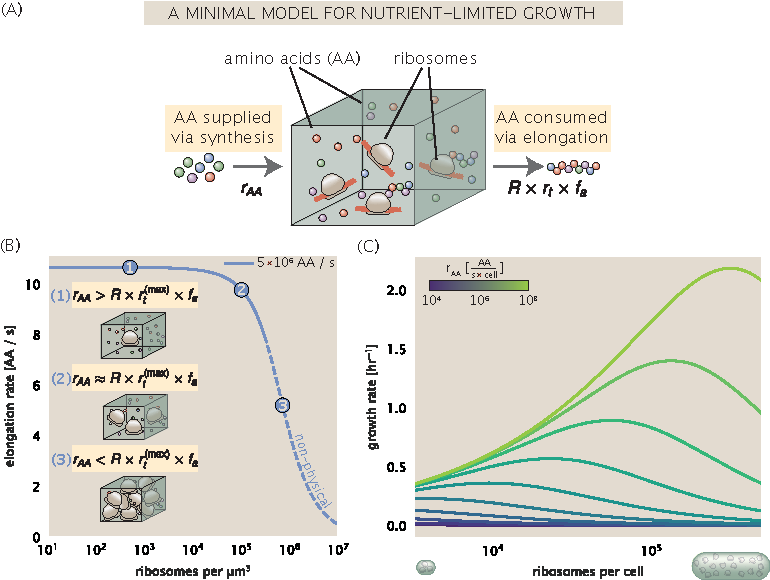
\includegraphics{main_figs/elongation_model.pdf}
        \caption{\textbf{A minimal model for regulation of growth rate under
        nutrient limitation.} (A) We consider a unit volume of cellular material
        composed of amino acids (colored spheres) provided at a supply rate
        $r_{AA}$. These amino acids are polymerized by a pool of ribosomes
        (brown blobs) at a rate $r_t \times R \times f_a$, where $r_t$ is the
        elongation rate, $R$ is the ribosome copy number in the unit volume, and
        $f_a$ is the fraction of those ribosomes actively translating. (B) The
        observed elongation rate is plotted as a function of ribosomes in a unit
        volume \textmu m$^3$. The three points correspond to three regimes of
        ribosome copy numbers and are shown schematically on the left-hand side.
        The region of the curve shown as dashed lines represents a non-physical
        copy number, but is shown for illustrative purposes. This curve was
        generated using the parameters $r_{AA} = 5 \times 10^6$ AA / s, $K_D =
        5$ mM, and $r_t^\text{(max)} = 17.1$ AA / s. (C) The cellular growth
        rate is plotted as a function of total cellular ribosome copy number for
        different cellular amino acid supply rates, with blue and green curves
        corresponding to low and high supply rates, repsectively. As the
        ribosome copy number is increased, so too is the cell volume and total
        protein abundance. We direct the reader to the Suppemental Information
        for discussion  on the inference of the realtionship between cell
        volume, number of peptide bonds, and ribosome copy number.}
        \label{fig:elongation_rate_model}
    }
\end{figure}

\subsubsection{Optimal Growth Rate, Ribosomal Content, and Cell Size Depend on Nutrient
Availability and Metabolic Capacity.}

To relate the elongation rate to growth rate, we will constrain  the set of parameters based
on the growth-rate dependent proteomic changes in the available data under
nutrient limitation;  namely, we will restrict the values of $R$, $N_{pep}$, and
$V$ to those associated with the growth conditions observed in the amalgamated 
proteomic data. We will then consider how changes in the nutrient conditions, through the parameter
$r_{AA}$, influence the maximum growth rate. 

Earlier, we codified our determination of ribosome biosynthesis as the
growth-rate determining cellular process in \EQ{lambda_limit} by stating that
the cellular growth rate $\lambda$ was related to the ribosome abundance,
elongation rate, active ribosome fraction, and the total number of peptide
bonds to be formed, $N_\text{pep}$. We return to this limit in light of our
expression for a condition-dependent elongation rate $r_t$ given by
\EQ{rt_root}. \FIG{elongation_rate_model}(C) shows how the observed growth
rate depends on the rate of amino acid supply $r_{AA}$ as a function of the
cellular ribosome copy number. A feature immediately apparent is the presence
of a maximal growth rate whose dependence on $R$ (and consequently, the cell
volume) increases with increasing
$r_{AA}$. Importantly, however, there is an optimum set of $R$, $N_{pep}$, and
$V$ that are strictly dependent on the value of $r_{AA}$. Increasing the
ribosomal concentration beyond the cell's metabolic capacity has the adverse
consequence of depleting the supply of amino acids and a concomitant decrease
in the elongation rate $r_t$ [\FIG{translation_model}(B)].

Of particular note is the growth rate profiles shown for low amino acid supply
rates [purple and blue lines in \FIG{elongation_rate_model}(C)], representing
growth in nutrient-poor media. In these conditions, there no longer exists a
peak in growth, at least in the range of physiologically-relevant  ribosome copy
numbers, indicating that when conditions are particularly poor, growth can be
increased by maintaining a minimal pool of active ribosomes. Depleting the
ribosome pool therefore permits resources to be devoted to maintaining metabolic
functions that can supply enough amino acids such that the ribosomes are
elongating at a maximal rate. This observation is in agreement with the central
with the central premise of the cellular resource allocation principle proposed
by \cite{scott2010, klumpp2009,klumpp2014, hui2015}.


%
%
% \subsubsection{\textit{E. coli} Maintains Growth in Poor Nutrient Conditions by a
% Reduction of Translation Activity.}
%
% In the slowest growth condition considered in the proteomic data, cells were
% grown in a chemostat ($\lambda$ = 0.12 hr$^{-1}$), and were found to have a ribosomal
% mass fraction of $\Phi_R \approx 0.06$ and of order 10$^4$ ribosomes per cell.
% In this absence of any additional regulation, we would predict a very low elongation rate of $r_t = X aa/s$.
%
% In contrast, wild-type \textit{E. coli} maintain a relatively high
% elongation rate even in stationary phase ($\approx$ 8 AA/s, \citep{dai2016,
% dai2018}).
%
% Careful
%
%
% In \FIG{}(B), we see that in the poorest nutrient conditions
% [NB: start by highlighting the dilemma when cells have excess ribosomes].
%
% How do cells regulate protein synthesis when amino acids become limiting,
% meaning that consumption exceeds the rate of synthesis? In the slowest  growth
% conditions, we find a minimum ribosomal mass fraction of $\Phi_R \approx 0.06$
% and  of order 10$^4$ ribosomes per cell.  Without the additional regulatory
% control noted above, there would be a point where  this imbalance would occur if
% all ribosomes were actively translating  (\FIG{translation_ecoli_partB}).
%
% Such a
% scenario would prevent continuous growth, and indeed for (p)ppGpp null strains,
% cells only grow in minimal media if additional amino acid supplements are
% present. In contrast, wild-type \textit{E. coli} maintain a relatively high
% elongation rate even in stationary phase ($\approx$ 8 AA/s, \citep{dai2016,
% dai2018}).
%
% To better understand how regulation of ribosomes influence growth rate at
% slow growth, we consider a coarse-grained model that relates elongation
% rate to a limiting supply of amino acids, which for simplicity we treat as a
% single, effective rate-limiting species $[AA]_{eff}$. Under such a scenario, the elongation
% rate $r_t$ can be described as depending on the maximum elongation rate ($r_t^{max}
% \approx$ 17.1 AA/s, \citep{dai2016, dai2018}), an effective binding constant
% $K_D$ between the pool of amino acids and their amino-acyl tRNAs, and the limiting
% amino acid concentration $[AA]_{eff}$,
%
% \begin{equation}
% r_t = r_t^{max} \cdot \frac{1}{1 + K_D / [AA]_{eff}}.
% \label{eq:rate_Kd}
% \end{equation}
% For cells growing in minimal medium supplemented with glucose, the amino acid
% concentration is of order 100 mM (BNID: 110093, \citep{milo2010, bennett2009}).
% To estimate  $K_D$, we note that for a growth rate of about 0.6 hr$^{-1}$
% \cite{dai2016} measured an elongation rate of about 12.5 AA$\cdot$s$^{-1}$,
% yielding $K_D \approx 40$ mM. The maintenance of this amino acid pool
% $[AA]_{eff}$ will depend on the difference between the synthesis/supply rate of
% amino acids $r_{AA}$ and consumption by ribosomes $r_t \times R \times f_a$,
% where we use $f_a$ to account for the possible reduction of actively translating
% ribosomes (see Supplemental Appendix XX for further details on this model).
%
% In \FIG{translation_ecoli_partB}(B), we show the relationship between the growth
% rate and elongation rate as a function of the number of actively translating
% ribosomes. Here, growth rate is now determined by the active ribosomal fraction via
% \begin{equation}
% \lambda_\text{translation-limited} \approx \frac{r_t}{L_R}  \Phi_R f_a.
% \label{eq:translation_limit_growth_rate_2}
% \end{equation}
% If we consider constant values of amino acid synthesis rate $r_{AA}$ (dashed
% lines) to reflect the available parameter space for a specific growth condition,
% the fastest growth rates result from  maximization of the fraction of actively translating
% ribosomes. When we consider the experimental measurements from \cite{dai2018}
% (yellow circles), reflecting growth in different nutrient conditions, we see
% that although $R \times f_a$ is reduced in poorer nutrient conditions, it is
% reduced in a manner such that $[AA]_{eff}$ is relatively constant. Given our estimate
% $K_D \approx$ 40 mM,  we would only expect a decrease from 100 mM to about 35 mM
% in the slowest growth conditions. While experimental data is scarce, data from
% \cite{bennett2009} show that amino acid
% concentrations only decrease to about 60 mM for cells grown in minimal media
% supplemented with acetate ($\lambda \approx$  0.3 hr$^{-1}$ in our proteomic data)
% \citep{bennett2009}, qualitatively consistent with our expectations. One
% explanation for the experimental data is that the active fraction of the
% ribosome pool is regulated in order to maintain a sufficient supply of amino acids for
% growth. Any further increase in $R \times f_a$ at constant $r_{AA}$ would
% otherwise be associated with an additional drop in cellular amino acid
% concentration.
%
% \begin{figure*}
%     \begin{fullwidth}
%     \centering{
%         \includegraphics{main_figs/fig8_ribosome_growth_limit_ecoli_b_2.pdf}
%         \caption{\textbf{\textit{E. coli} must regulate ribosomal activity in
%         limiting nutrient conditions. }
%         (A) Translation elongation rate is plotted
%         as a function of the number of actively translating ribosomes $R
%         f_a$. Dashed lines correspond to a range of amino acid synthesis rates
%         $r_{aa}$, from 10$^3$ to 10$^6$. Growth rates are calculated according
%         to Equation 1, assuming a constant ribosomal fraction of 8 percent. See
%         appendix XX for additional details.}
%         \label{fig:translation_ecoli_partB}
%     }
%     \end{fullwidth}
% \end{figure*}
%

%
% [important point is that as resources become limiting, cells are able to tune and minimize
% the entire cell mass - which enables them to grow faster]
%
% [Discuss implications of findings so far. All other components being tuned (mostly) in the required proportions; and also that the achievable growth rate is ultimately set by ribosomes. ]
%
% [The apparent constraint that cells MUST get larger in order to grow faster places a particular constrain on why a cell would vary its ribosomal fraction in the first place.]
%
% [Also present the evidence from literature that there is a prominent role for aa/nutrient sensing that appears to mediate X, Y, and Z. ]
%
% [Then go on to propose the way to understand what’s going on with our model.
%     - I think maybe it’s easiest to understand it is we start by considering the balance that must be maintained between metabolic activity and ribosomal activity.
%     - Then write down a model that relates how elongation rate will relate to this.]
%
%
%

% [Figure idea: PART (A) Maybe we can consider that r_t*R sets the maximum rate of growth; but you also need to feed that engine and build the house to fit them.]
%
% [ When I get into slow growth regime; consider that IF R scales with <#ori>, ribosomes will have increasingly longer wait times for protein synthesis. Which is bad.
%     - By also decreasing the fraction of actively translating ribosomes, cells can grow faster is also super important. ]
%
%
%
%
